\documentclass[12pt]{article}

\input preamble

\title{Principles of Parallel Architecture\\
Project Report 3}
\author{Xitong Liu \\
xliu@ece.udel.edu}

\begin{document}

\maketitle

\section{Introduction}
In this report, we will introduce more optimization methods applied
to parallel matrix multiplication. At last, we will report the 
performance in different aspect in detail.

\section{Instruction Level Parallelism}
Instruction level Parallelism is one of the most useful techniques which
can be applied to improve the performance of parallel program greatly.
In this program, we use gcc to generate the assembly code of the method
which performs best in methods we proposed in the last report. Then we
adjust the instructions as well as the instruction order to reach the
best performance. Several methods were applied:

\begin{enumerate}
\item \textbf{Register Renaming}: reduce the data dependencies between 
the adjacent instructions.
\item \textbf{Instruction Pipelining}: utilize the pipeline of the 
processor to hide the latency of data loading and storing from and to 
the memory.
\item \textbf{Out of Order Execution}: hide the loading and storing 
latency in instructions without data dependency.
\end{enumerate}

During the optimization process, we found some interesting facts from
the assembly code generated by gcc. To our surprise, gcc generates the
instructions in a na\"\i ve way which is inefficient. Here is an example:

\scriptsize
\begin{verbatim}
#oprand_b_0 = __builtin_ia32_loadups(&(matrixBT.data[cycleJ * dim + cycleK]));
	movq	-248(%rbp), %rax
	movq	16(%rax), %rax
	movq	(%rax), %rdx
	movq	-248(%rbp), %rax
	movl	32(%rax), %eax
	imull	-20(%rbp), %eax
	addl	-24(%rbp), %eax
	cltq
	salq	$2, %rax
	leaq	(%rdx,%rax), %rax
	movups	(%rax), %xmm0
	movlps	%xmm0, -192(%rbp)
	movhps	%xmm0, -184(%rbp)       #%xmm0 -> oprand_b_0

#oprand_b_0 = __builtin_ia32_loadups(&(matrixBT.data[(cycleJ  + 1)* dim + cycleK]));
	movq	-248(%rbp), %rax
	movq	16(%rax), %rax
	movq	(%rax), %rdx
	movl	-20(%rbp), %eax
	leal	1(%rax), %ecx
	movq	-248(%rbp), %rax
	movl	32(%rax), %eax
	imull	%ecx, %eax
	addl	-24(%rbp), %eax
	cltq
	salq	$2, %rax
	leaq	(%rdx,%rax), %rax
	movups	(%rax), %xmm0
	movlps	%xmm0, -208(%rbp)
	movhps	%xmm0, -200(%rbp)       #%xmm0 -> oprand_b_1
	
#oprand_b_0 = __builtin_ia32_loadups(&(matrixBT.data[(cycleJ + 2) * dim + cycleK]));
	movq	-248(%rbp), %rax
	movq	16(%rax), %rax
	movq	(%rax), %rdx
	movl	-20(%rbp), %eax
	leal	2(%rax), %ecx
	movq	-248(%rbp), %rax
	movl	32(%rax), %eax
	imull	%ecx, %eax
	addl	-24(%rbp), %eax
	cltq
	salq	$2, %rax
	leaq	(%rdx,%rax), %rax
	movups	(%rax), %xmm0
	movlps	%xmm0, -224(%rbp)
	movhps	%xmm0, -216(%rbp)       #%xmm0 -> oprand_b_2
\end{verbatim}
\normalsize

In this example, the index of the matrix data array is calculated from 
scratch each time to load four numbers to the vector which lead to 
unnecessary and duplicate instruction execution. Actually there is a 
fixed stride (\texttt{dim}) between the indices. So we can calculate 
the index at the first load and increase the index by \texttt{dim} in 
the following loads which may save a lot of instructions. The optimized
code is shown as below:

\scriptsize
\begin{verbatim}
# dim -> %rcx
	movq	-248(%rbp), %rax
	movl	32(%rax), %eax
	cltq
	mov     %rax, %rcx
  
#matrixRT.data -> %rdx
	movq	-248(%rbp), %rax
	movq	16(%rax), %rax
	movq	(%rax), %rdx

#oprand_b_0 = __builtin_ia32_loadups(&(matrixBT.data[cycleJ * dim + cycleK]));
        
# (cycleJ * dim + cycleK) -> %rsi
	movl    %ecx, %eax
	imull	-20(%rbp), %eax         #-20(%rbp) is cycleJ
	addl	-24(%rbp), %eax
	cltq
        
	mov     %rax, %rsi
	add     %rcx, %rsi
	
	salq	$2, %rax
	leaq	(%rdx,%rax), %rax
	movups	(%rax), %xmm0
	movlps	%xmm0, -192(%rbp)
	movhps	%xmm0, -184(%rbp)       #%xmm0 -> oprand_b_0

#oprand_b_1 = __builtin_ia32_loadups(&(matrixBT.data[(cycleJ  + 1)* dim + cycleK]));
	mov     %rsi, %rax
	add     %rcx, %rsi

	salq	$2, %rax
	leaq	(%rdx,%rax), %rax
	movups	(%rax), %xmm0
	movlps	%xmm0, -192(%rbp)
	movhps	%xmm0, -184(%rbp)       #%xmm0 -> oprand_b_0

#oprand_b_2 = __builtin_ia32_loadups(&(matrixBT.data[(cycleJ + 2) * dim + cycleK]));
	mov     %rsi, %rax
	add     %rcx, %rsi

	salq	$2, %rax
	leaq	(%rdx,%rax), %rax
	movups	(%rax), %xmm0
	movlps	%xmm0, -192(%rbp)
	movhps	%xmm0, -184(%rbp)       #%xmm0 -> oprand_b_0


\end{verbatim}
\normalsize


\section{Experiment Results}
\subsection{Experiment Setup}
The matrix size is $1024\times 1024$ in float numbers and number of 
threads is 32. We apply different optimization methods step by step, 
and new optimization method is combined with the previous one. Since 
it's limited by the space, we assign different method combinations to 
different IDs, shown in Table~\ref{tab:methods}.

\begin{table}[h!]
	\small
	\begin{center}
	\caption{\label{tab:methods} Method Combinations ID Map}
	\begin{tabular}{|r|l|}
		\hline
		ID & Method Combination \\ \hline
		0 &	Serial \\ \hline
		1 & Baseline \\ \hline
    2 & Transpose \\ \hline
    3 & Transpose + SSE \\ \hline
    4 & Transpose + SSE + Unrolling (4 cycles) + Scheduling \\ \hline
    5 & Transpose + SSE + Unrolling (2 cycles) + Scheduling + 
      Software pipelining \\ \hline
    6 & Transpose + SSE + Unrolling (4 cycles) + Scheduling + ILP\\ \hline
	\end{tabular}
	\end{center}
\end{table}

\subsection{Results}
To explore the performances under different optimization settings by 
the compiler, we run the experiments in two groups: one with 
\texttt{-O3} option and the other without any optimization. For 
each setup, we run the program 20 times and calculate the average 
run time as the measurement of performance. The results are shown in 
Table~\ref{tab:performance}.

\begin{table}[h!]
	\small
	\begin{center}
	\caption{\label{tab:performance} Performance Comparison}
	\begin{tabular}{|r|r|r|r|r|}
		\hline
		 & \multicolumn{2}{c|}{NO Optimization} & \multicolumn{2}{c|}{-O3 Optimization} \\ \hline
		Method & Time(s) & Speed Up & Time(s) & Speed Up \\ \hline
		0  &  33.7776	& 1.0000		&19.4682		&	1.0000 \\ \hline
		1  &		4.5976		&	7.3468		& 2.3256		&	8.3712 \\ \hline
		2  &		4.1109  & 8.2166		&	0.4622		&	42.1209 \\ \hline
		3  &		0.9353  & 36.1142	&	0.4656		&	41.8133 \\ \hline
		4  &		0.6091  & \textbf{55.4550}	& 0.4208		&	\textbf {46.2649} \\ \hline
		5  &		0.7761  & 43.5223	&	0.4660		&	41.7774 \\ \hline
	\end{tabular}
	\end{center}
\end{table}

\subsection{Analysis}
Based on the observations in the results, we can draw the following interesting 
conclusions:
\begin{enumerate}
\item Our current best performance (Method 4) without any optimization has reached 
the 60\% of the best performance with -O3 optimization.
\end{enumerate}

\section{Conclusion}

\end{document}

\begin{comment}
\begin{figure}[h!]
	\begin{center}
		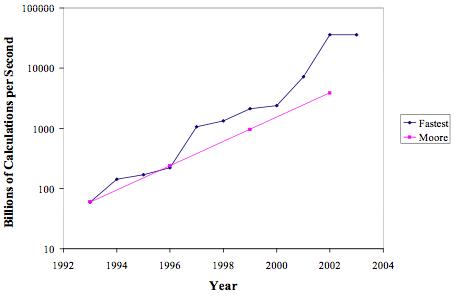
\includegraphics[width=0.7\textwidth, angle=0]{fatest.png}
		\caption{\label{fig:fatest}Fatest SuperComputer in the world}
	\end{center}
\end{figure}
\end{comment}